\documentclass{article}

\usepackage[T1]{fontenc}    %Schriftart des Dokumentes
\usepackage[ngerman]{babel} %Dokumentensprache, hier Deutsch
\usepackage{amsmath, amssymb, stmaryrd} %mathematische Schriftzeichen
\usepackage{graphicx} %Einfügen von Grafiken
\usepackage{wrapfig}
\usepackage{bm}

\setlength{\parindent}{0pt} %Einrückung von Absätzen auf null gesetzt
\setlength{\parskip}{10pt} %Abstand zischen Absätzen auf 10pt gesetzt

\title{Versuch 23: Strom- und Spannungsmessungen}
\author{Matthias Kuntz}
\date{29.09.2023}

\begin{document}

\maketitle

%-------------------------EINLEITUNG-------------------------
\section{Einleitung}

Elektrizität ist einer der wichtigsten Aspekte in allen Bereichen der modernen Welt. Von hochtechnischen Geräten in der Wissenschaft und Forschung bis hin zum alltäglichen Benutzen des Wasserkochers des morgentlichen Kaffees, nichts davon würde ohne Strom, ergo ohne die Elektrizität funktionieren. Somit ist es klar, dass im Anfängerpräktikum der Physik ein Versuch, bei dem die Grundlagen der Elektrizität über Strom- und Spannungsmessungen erarbeitet werden, auf keinen Fall fehlen darf, um ein Gefühl und ersten wissenschaftlichen Kontakt mit der fast schon fundamentalsten Grundlage des modernen Alltags zu bekommen.     

\subsection{Physikalische Grundlagen}

Wenn man alltäglich vom Strom spricht, so meint man damit meist die Transportation von elektrischen Ladungsträgern in einem leitenden Medium. Zunächst ist es angebracht Spannungsquellen zu betrachten. Diese lassen sich unterteilen in ideale und reale Spannungsquellen. Während bei den Idealen die ausgegebene Spannung $U$ einfach der Quellspannung $U_q$ entspricht, fällt bei einer realen Spannungsquelle die wirklich ausgegebene Klemmspannung mit zunehmender Stromstärke $I$. 

\begin{figure} [!h]
    \centering
    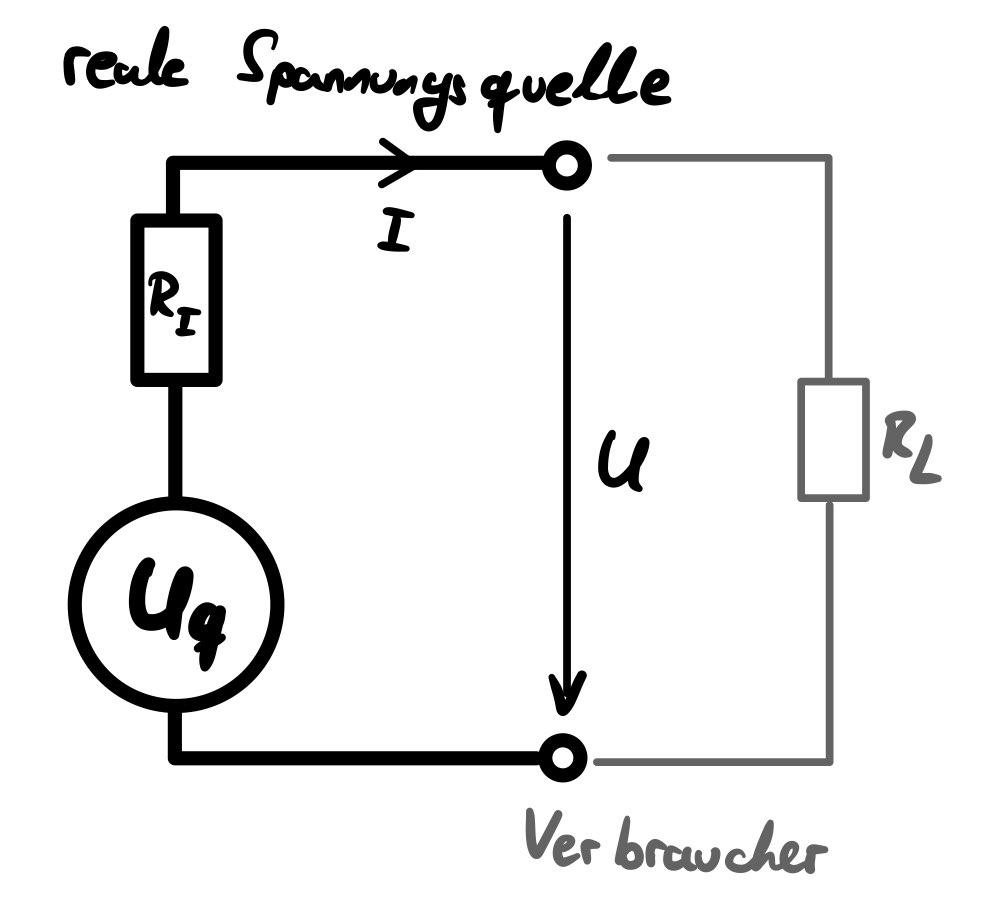
\includegraphics[width=5cm]{graphics/realspann.jpg}
    \caption{Reale Spannungsquelle mit Verbraucher}
    \label{fig:realspann}
\end{figure}

Bei sogenannten linearen Spannungsquellen ist die abfallende Spannung proportional zum Innenwiderstand $R_I$ der Spannungsquelle und kann bestimmt werden, indem den Innenwiderstand als zur Quelle in Reihe geschaltet betrachtet (siehe Abbildung \ref{fig:realspann}). Die Klemmspannung $U$ ist dann gegeben als

\begin{equation}
    U = U_q - R_I I.
\end{equation}

Schließt man an die reale Spannungsquelle nun einen Verbraucher in Form des Widerstands $R_L$ an, so fließt der Strom

\begin{equation}
    I = \frac{U_q}{R_I + R_L}
\end{equation}

hergeleitet aus dem Ohmschen Gesetz und für die Klemmspannung gilt:

\begin{equation}
    U = R_L I = U_q \frac{R_L}{R_I + R_L}
\end{equation}

Wir werden verschiedene Instrumente zum Messen von Strom und Spannung verwenden. Das Erste ist ein sogenanntes Drehspulinstrument. Mithilfe einer Spule, durch die der Strom geleitet wir, wird ein Magnetfeld erzeugt, dessen Stärke proportional zum angelegten Strom ist und einen Zeiger somit unterschiedlich stark ausschlagen lässt. Jedoch kann man bei bekannten Widerständen nicht nur die Stromstärke, sondern auch die anliegende Spannung messen. 

Hat man eine Reihenschaltung von realer Spannungsquelle mit Innenwiderstand $R_{Iq}$, Amperemeter, was auch einen Innenwiderstand $R_{Ia}$ hat, und dem Verbraucher mit Widerstand $R_L$, so fließt der Strom

\begin{equation}
    I = \frac{U_0}{R_L + R_{Iq} + R_{Ia}}.
\end{equation}

Damit ein Amperemeter also keinen Einfluss auf die gemessene Stromstärke hat, muss der Innenwiderstand von diesem möglichst gering sein.

Ein Spannungsmessgerät (Voltmeter) hingegen wird parallel zur Spannungsquelle und dem Verbraucher geschaltet. Der Innenwiderstand vom Voltmeter wird mit $R_{Iv}$ bezeichnet. Man erhält über die Kirchhoffschen Regeln bei so einem Aufbau die Spannung am Verbraucher als

\begin{equation}
    U = U_q \frac{R_L}{\frac{R_{Iq}R_{L}}{R_{Iv}} + R_{Iq} + R_L}.
\end{equation}

Im Gegensatz zum Amperemeter muss also der Innenwiderstand des Voltmeters möglichst groß sein um die Spannung am Verbraucher nicht zu beeinflussen.

Das zweite verwendete Messinstrument ist ein Kompensator. Der schematische Aufbau ist in Abbildung \ref{fig:kompensator} gezeigt. Es funktioniert, indem man eine bekannte Spannung, in unserem Fall sind das 6V, anlegt und die Skala des Instruments zunächst auf eine Eichspannung eicht. Dazu variiert man den Eichregler, einen verstellbaren Widerstand, bis am Amperemeter eine Spannung von 0 anliegt. Das Drehpotentiometer ist dabei mit einer Skala verbunden und der auf der Skala angezeigte Wert entspricht dann der geeichten Spannung. Legt man nun eine beliebige Spannung innerhalb der Skalenreichweite an, so kann man, indem man nun mit den Drehpotentiometer den Widerstand variiert und den Eichregler unberührt lässt den gemessenen Strom auf Null stellen und den an der Skala angezeigten Wert mithilfe des geeichten Werts in die gesuchte Spannung umrechnen.

\begin{figure} [!h]
    \centering
    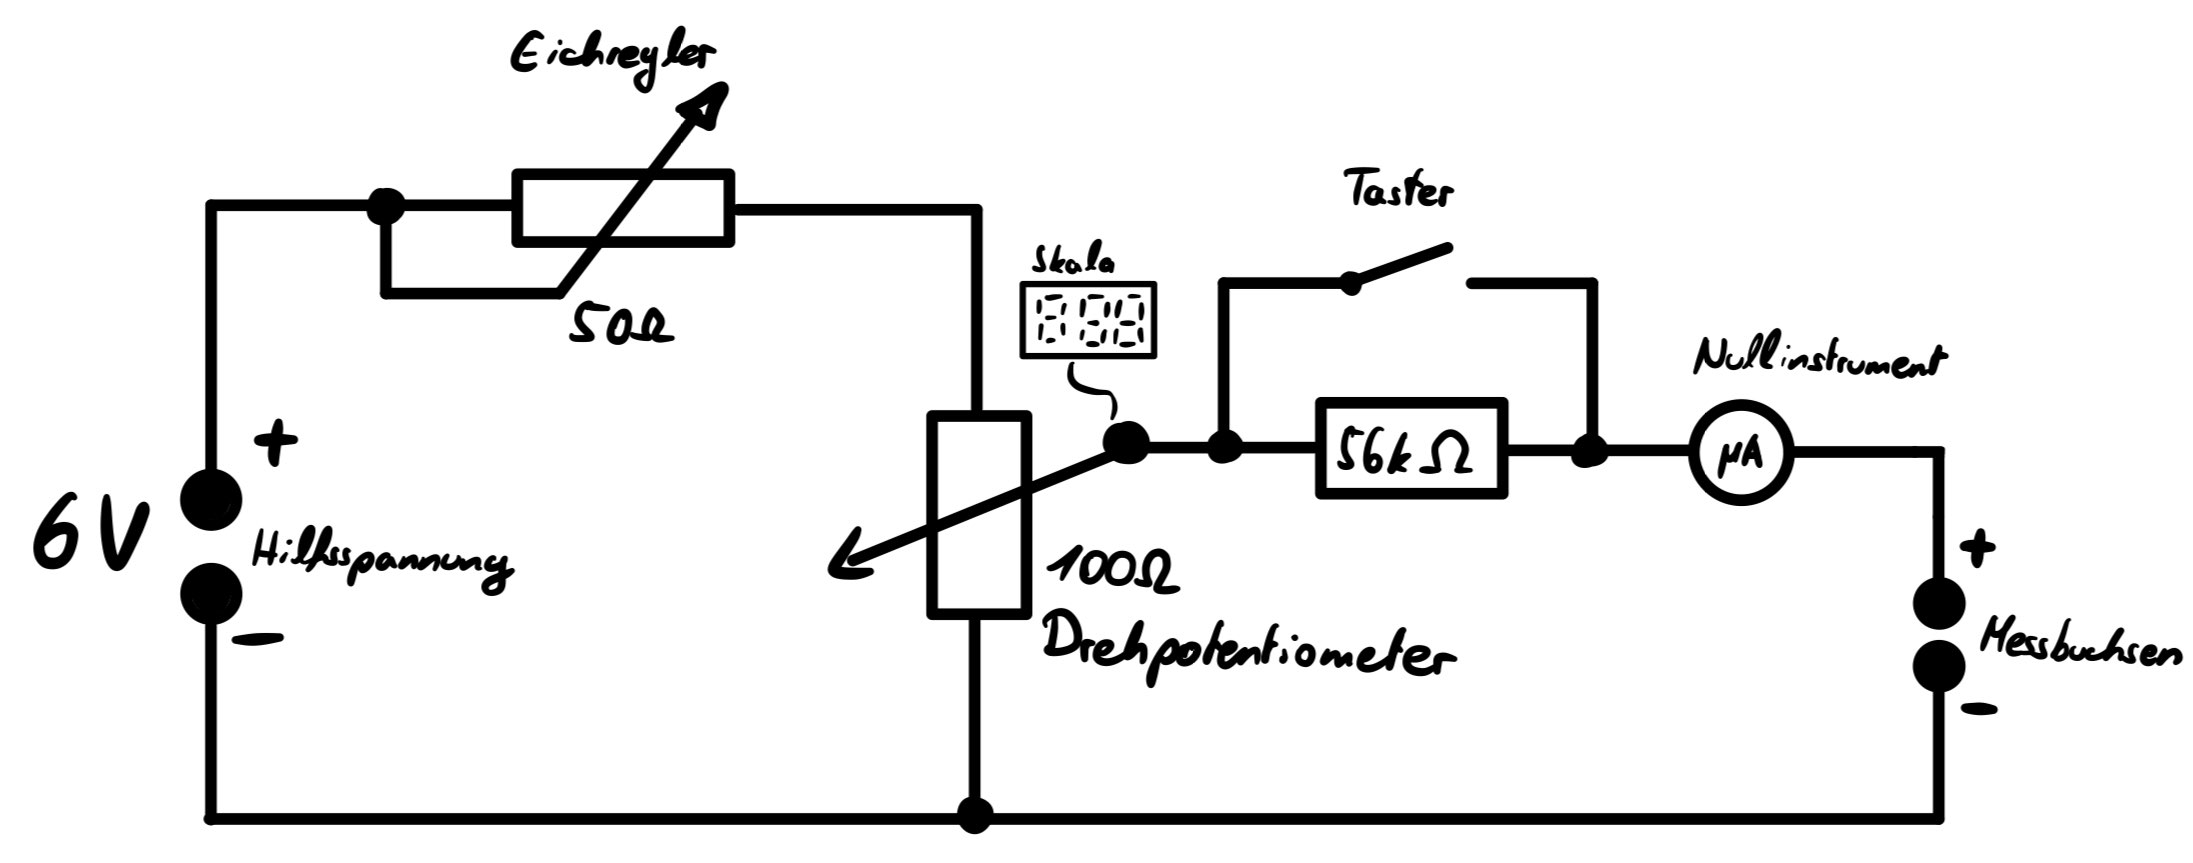
\includegraphics[width=11cm]{graphics/komp.jpg}
    \caption{Aufbau eines Kompensators}
    \label{fig:kompensator}
\end{figure}

Der Vorteil des Kompensator ist hierbei, dass bei der Kompensation kein Strom fließt, da dieser ja auf null gestellt wird, und somit der Innenwiderstand automatisch sehr hoch ist.

\newpage

Möchte man den Messbereich eines Messinstruments um den Faktor $f$ erweitern, so geht das, indem man Widerstände paralell oder in Reihe dazu schaltet. Beim Amperemeter mit Innenwiderstand $R_{Ia}$ muss der Widerstand

\begin{equation}
    R_p = \frac{R_{Ia}}{f-1}
\end{equation}

parallel geschaltet werden. Beim Voltmeter, Innenwiderstand $R_{Iv}$, muss der Widerstand

\begin{equation}
    R_s = R_{Iv}(f-1)
\end{equation}

in Serie geschaltet werden.

\subsection{Versuchsaufbau}

In diesem Versuch werden verschiedene Messungen mit verschiedenen Instrumenten durchgeführt. Wir beginnen mit dem Eichen des Kompensators, wofür wir die 2,5V Eichspannung an diesen anschließen. \\
Anschließend bauen wir den Schaltkreis in Skizze 2 im Messprotokoll auf, um das Drehspulinstrument als Voltmeter zu verwenden. \\
Zuletzt machen wir den Aufbau in Skizze 3 und Messen mit dem Kompensator die Spannung und mit dem Drehspulinstrument den Strom aus der Batterie bei unterschiedlichen Positionen des Schiebewiderstands. 


%---------------VERSUCHSPROTOKOLL MIT MESSDATEN---------------
\newpage

\section{Versuchsprotokoll mit Messdaten}

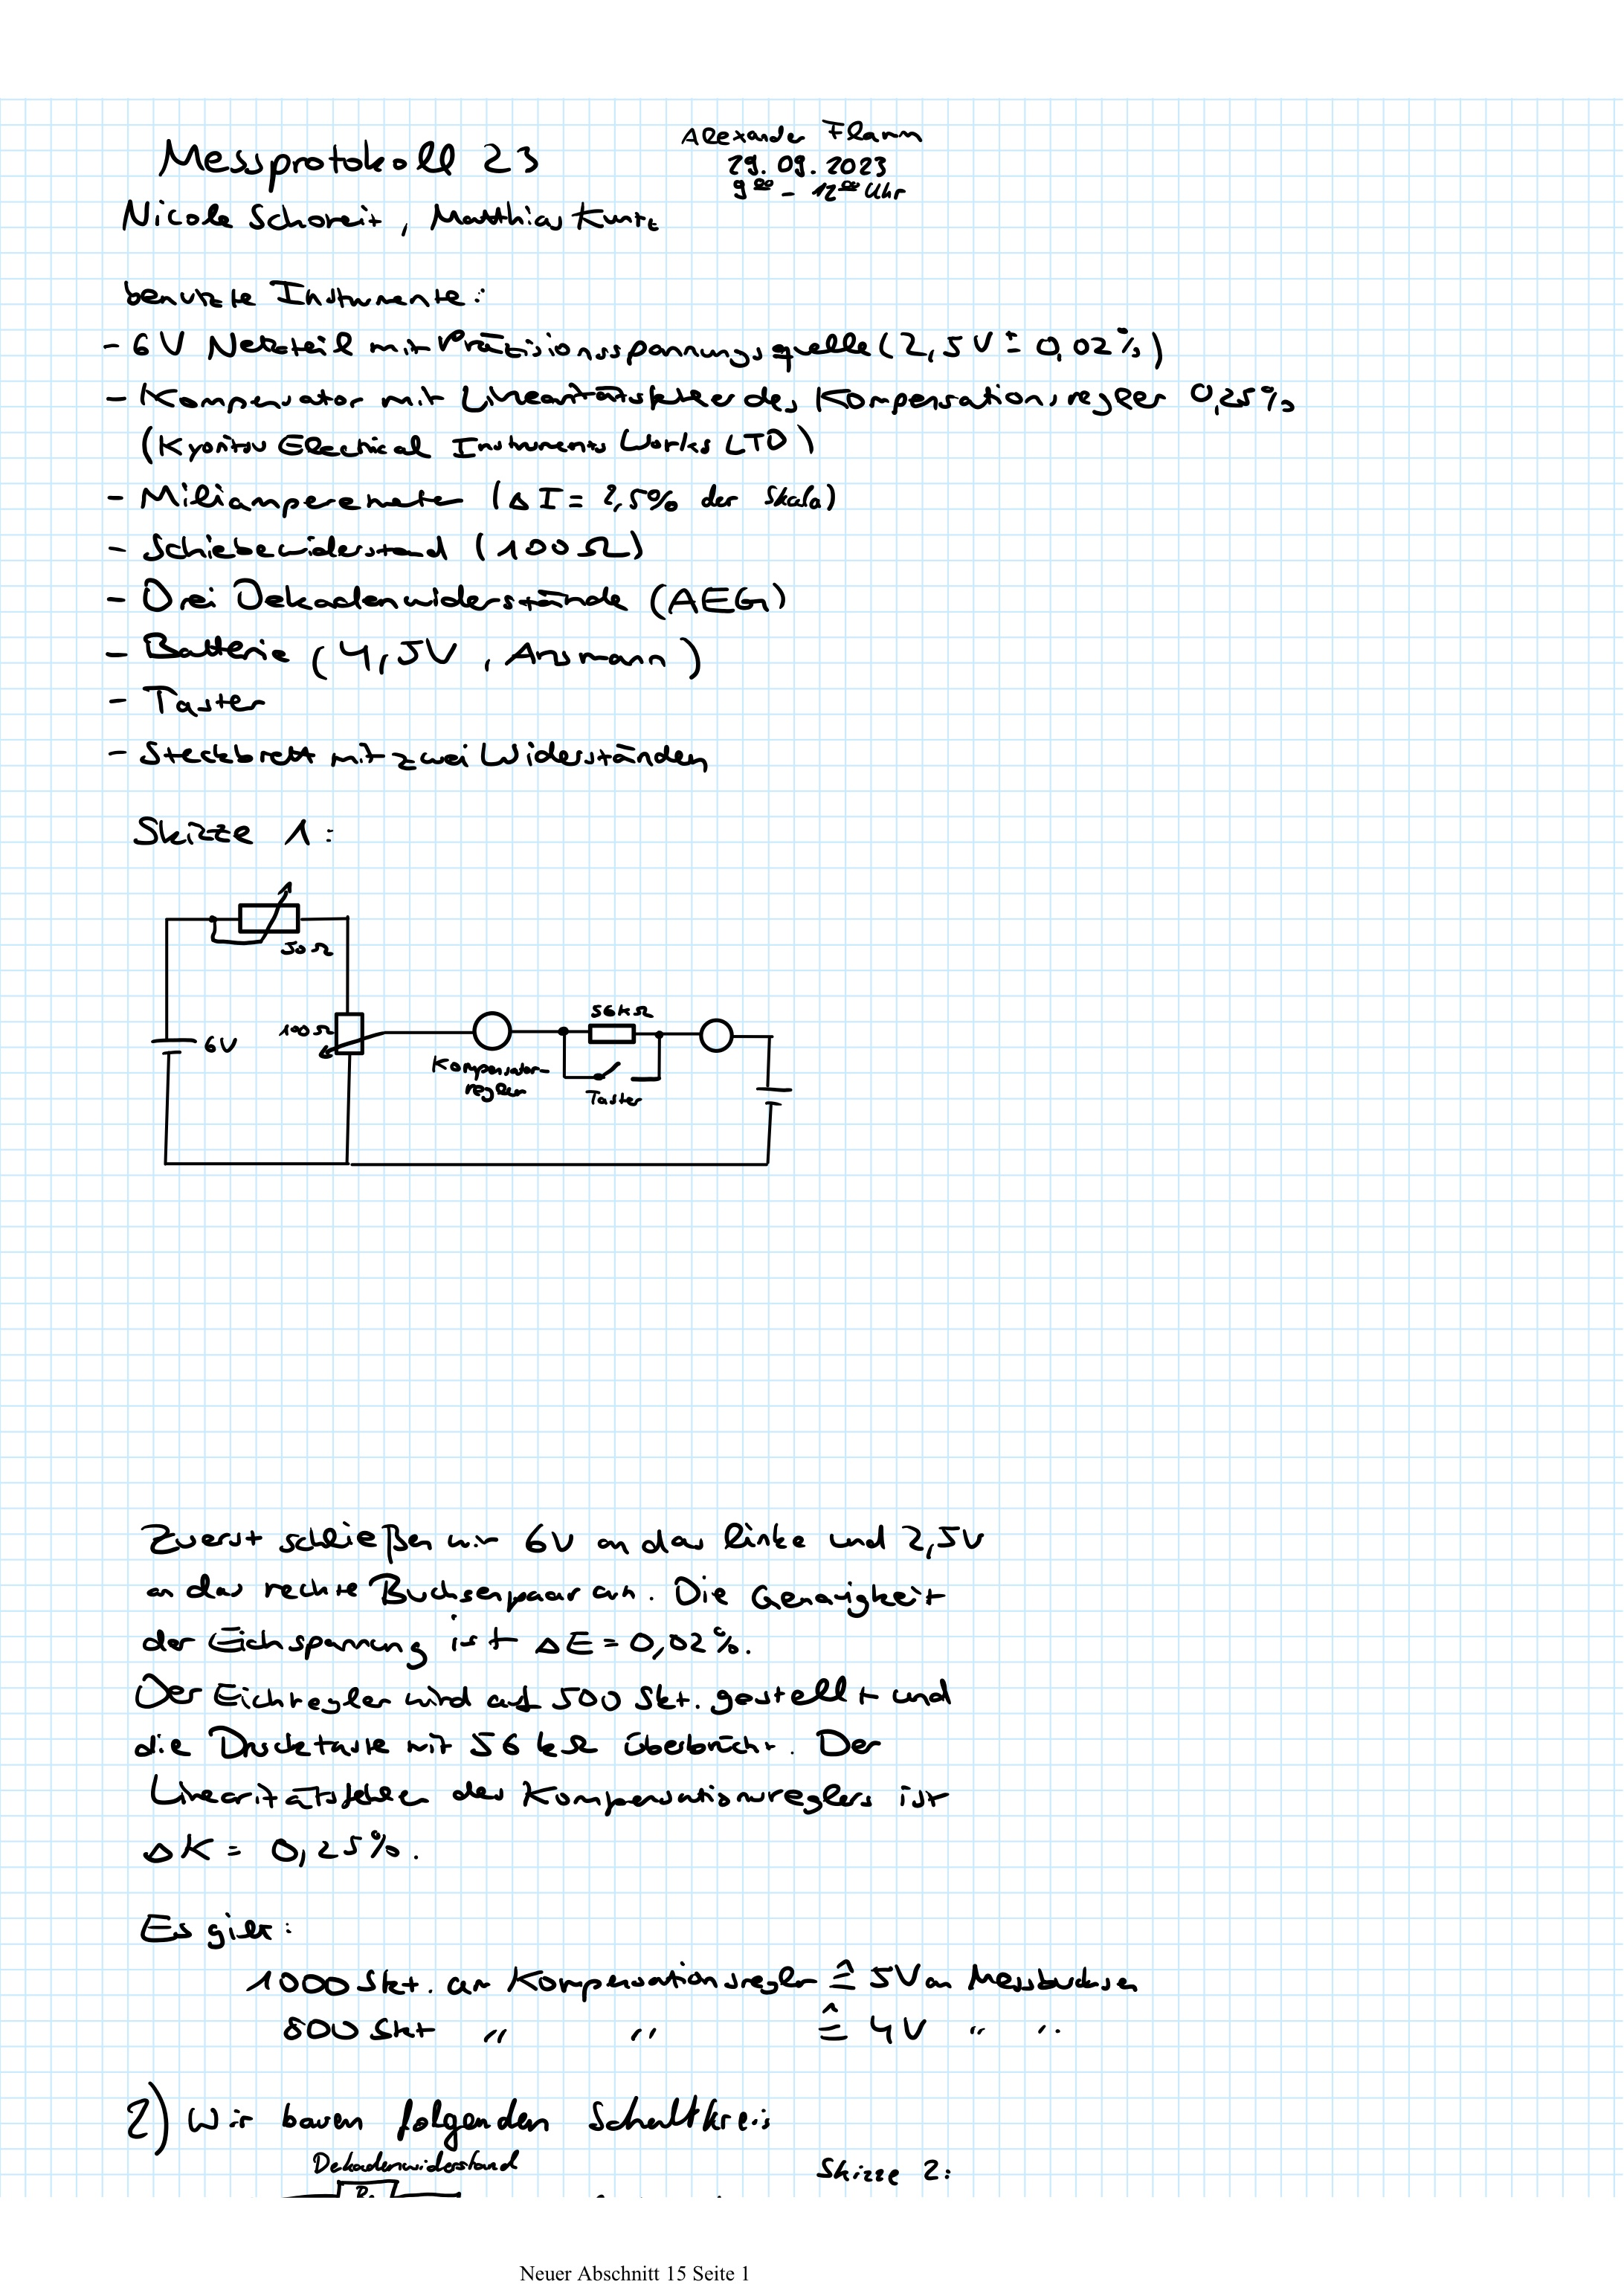
\includegraphics[width=\textwidth]{graphics/mess1.jpg}
\newpage
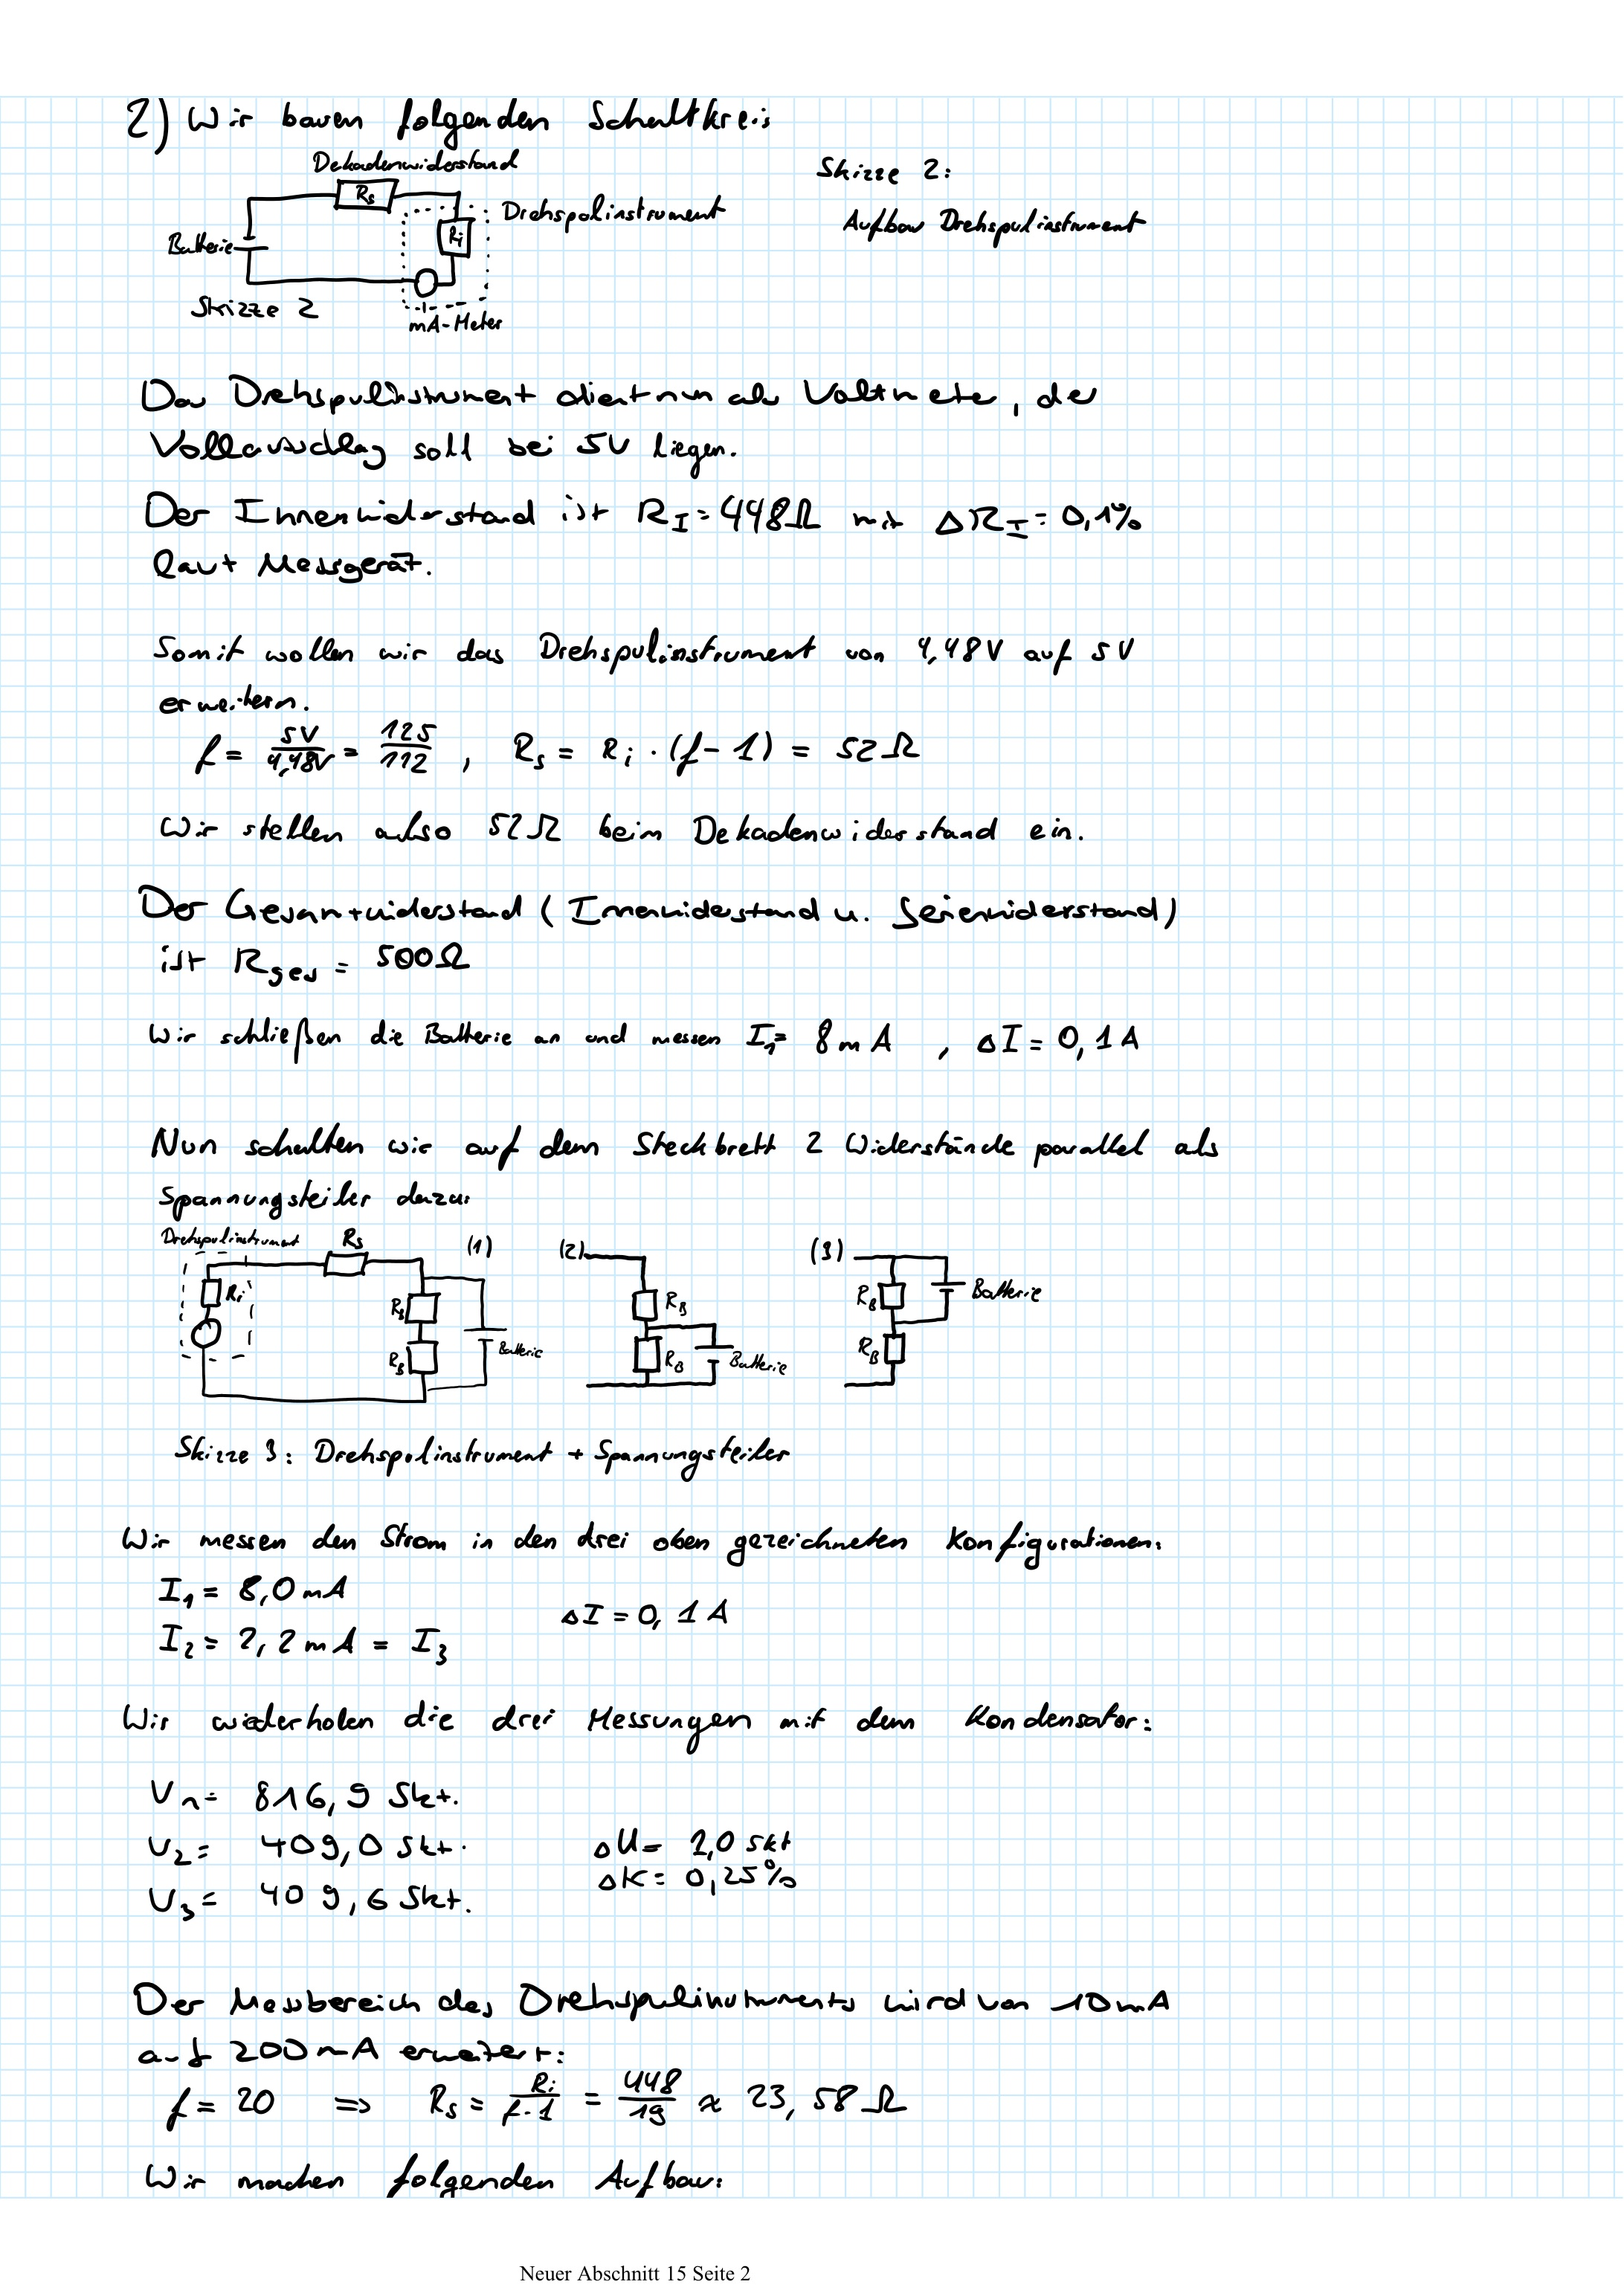
\includegraphics[width=\textwidth]{graphics/mess2.jpg}
\newpage
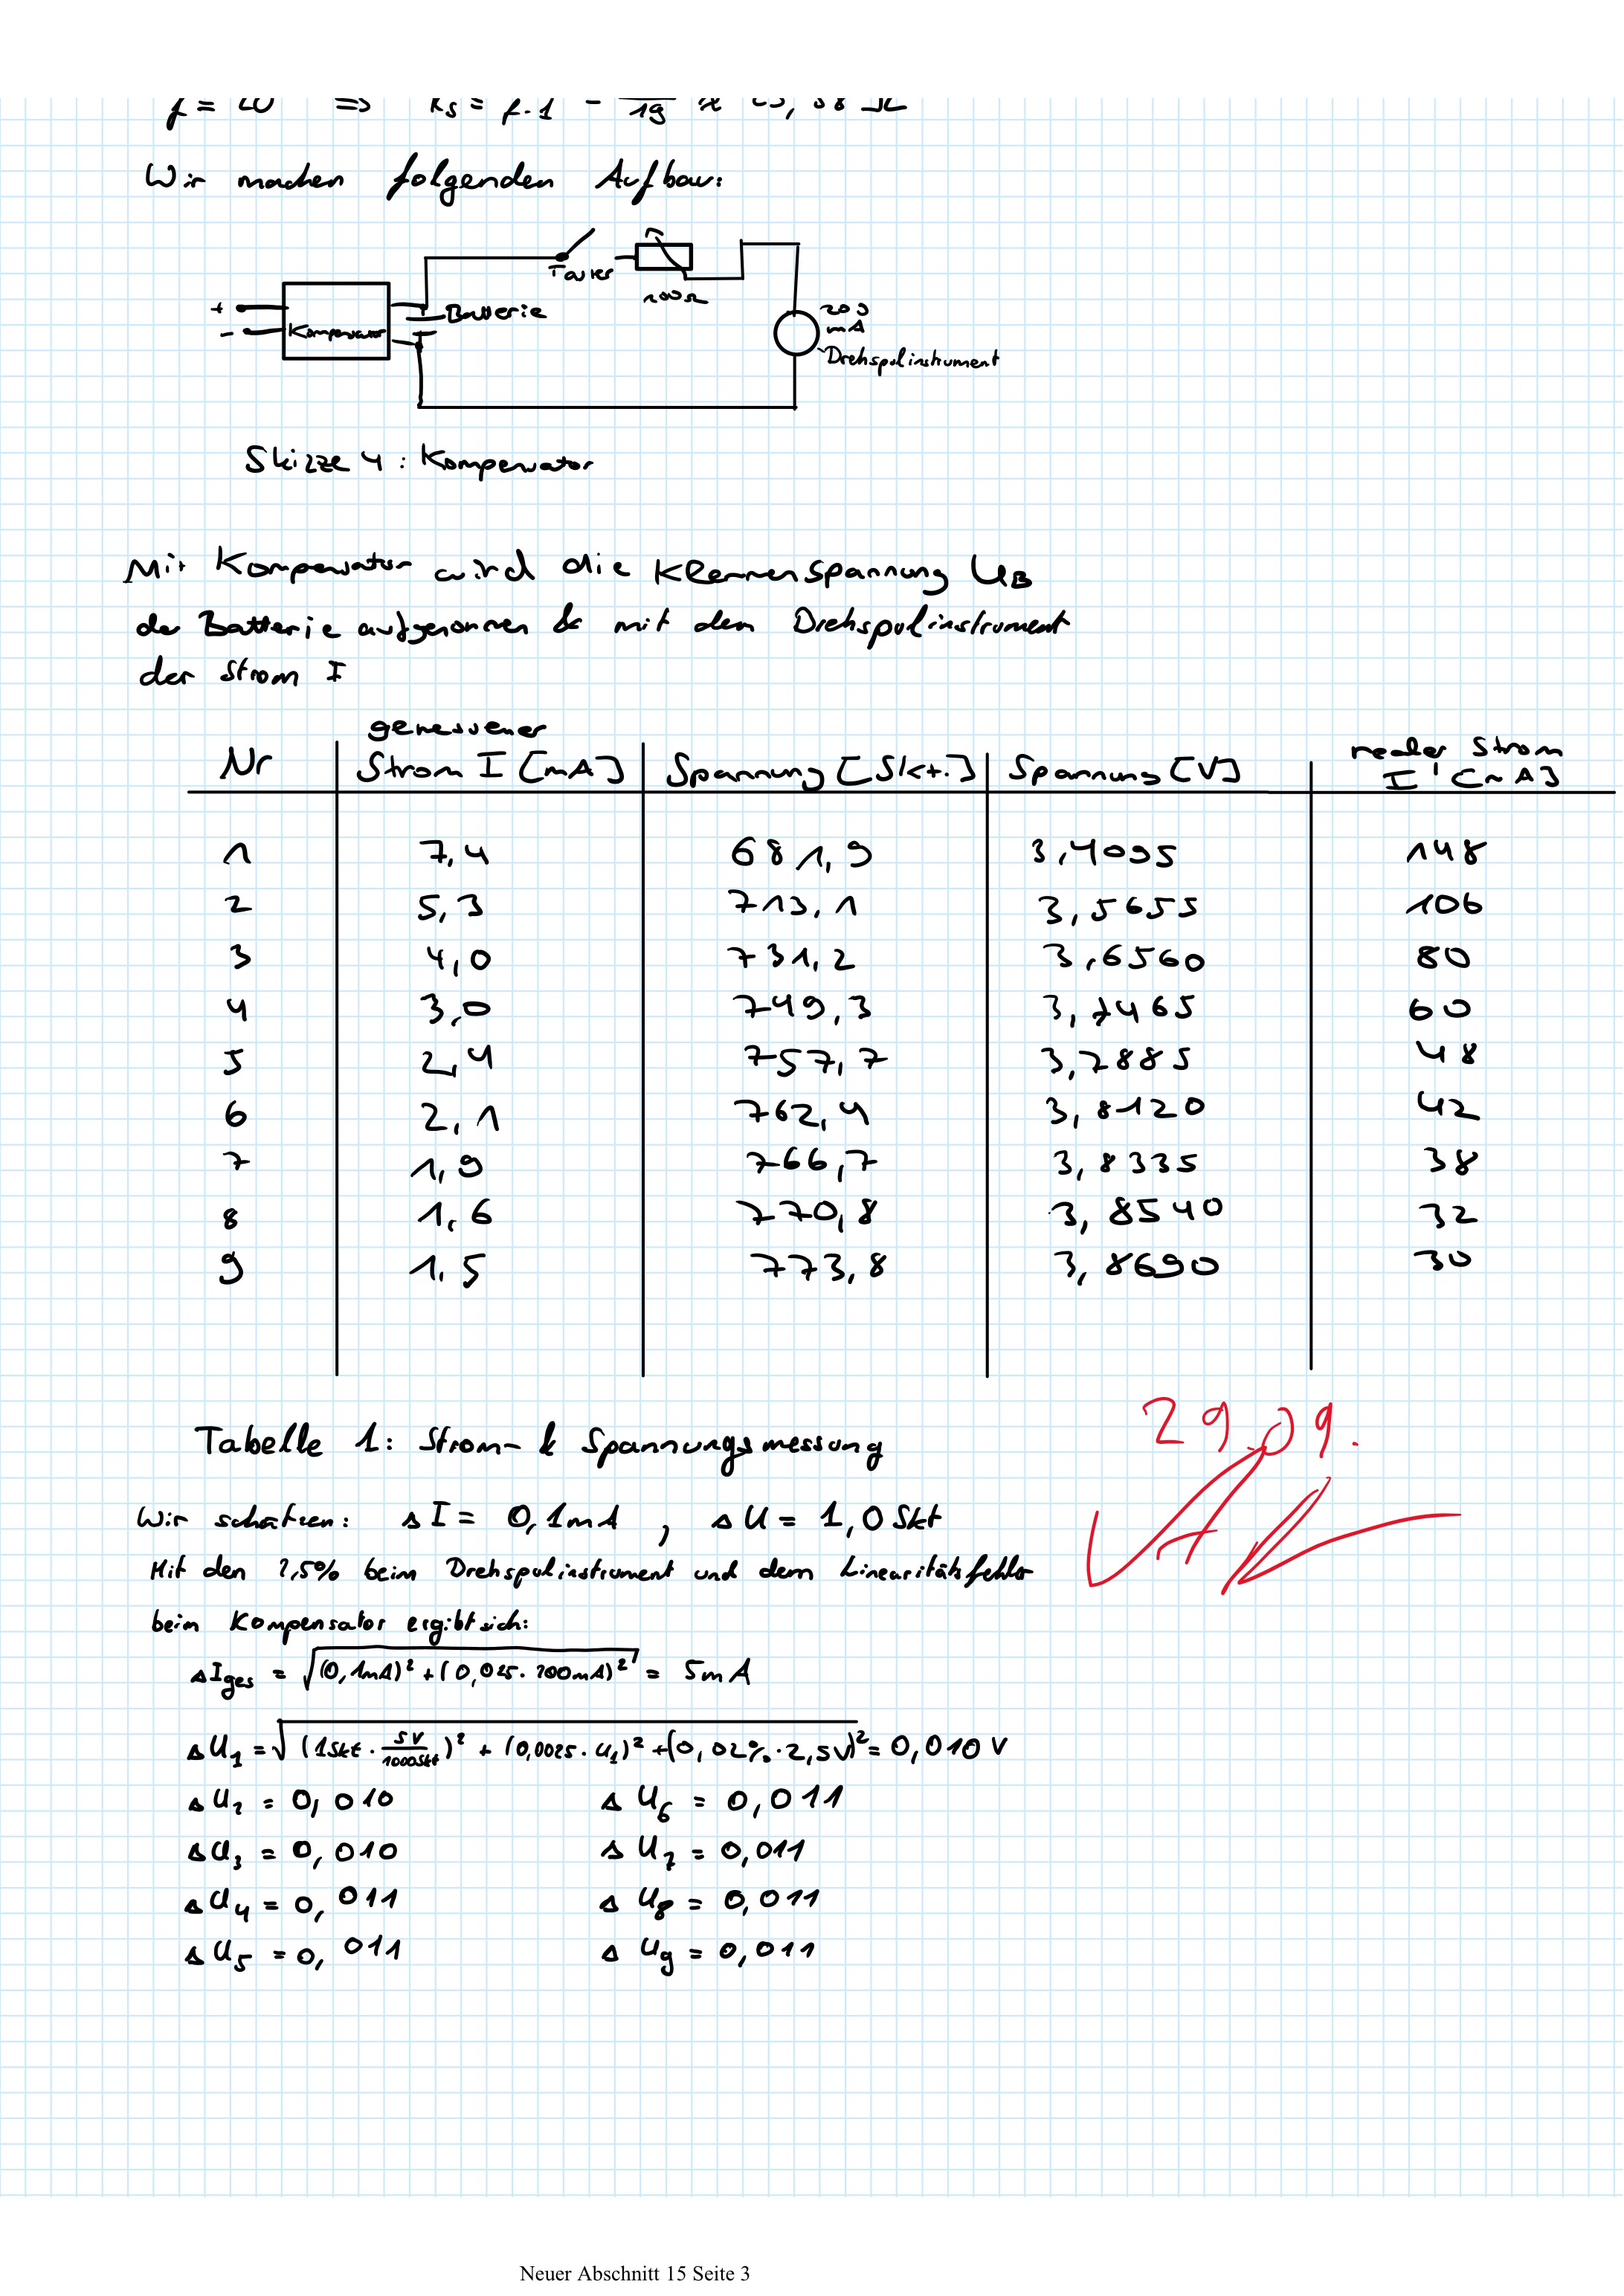
\includegraphics[width=\textwidth]{graphics/mess3.jpg}
\newpage

\addtocounter{table}{1}

%-------------------------AUSWERTUNG-------------------------
\section{Auswertung}

In dieser Evaluation werden alle Fehler, sofern keine spezifische Angabe gemacht wird, mithilfe der Gauss'schen Fehlerfortpflanzung berechnet. Dies bedeutet, dass ein Wert $F$, der mit der Formel $f(a_1, ..., a_n)$ berechnet wird, den Fehler $\Delta F$ gegeben über folgende Formel hat:

\begin{equation}
    \Delta F = \sqrt{\sum_n \left( \frac{\partial f}{\partial a_n} \cdot \Delta a_n \right)^2}.
\end{equation}

\subsection{Auswertung der Messungen bei Erweiterung auf 5V}

Wir beginnen, indem wir aus den gemessenen Angaben vom Drehspulinstrument und dem Kompensator die wirklich gemessenen Spannung berechnen. Wir kennzeichnen die Spannungen vom Drehspuhlinstrument mit dem Index $d$ und die des Kompensators mit $k$. Der Fehler der Spannungen mit dem Kondensator setzt sich hierbei zusammen aus dem Messfehler der Skalenteile, dem Linearitätsfehler der Skala sowie dem Fehler der Eichspannung:

\begin{equation}
    \begin{split}
        U_i^{(d)} &= I_i \cdot \frac{5\text{V}}{10\text{mA}} \\ 
        \Delta U_i^{(d)} &= \Delta I_i \cdot \frac{5\text{V}}{10\text{mA}} \\
    \end{split}
\end{equation}

\begin{equation}
    \begin{split}
        U_1^{(d)} &= (4,00 \pm 0,05) \text{V} \\
        U_2^{(d)} &= (1,10 \pm 0,05) \text{V} \\
        U_3^{(d)} &= (1,10 \pm 0,05) \text{V} 
    \end{split}
\end{equation}

\begin{equation}
    \begin{split}
        U_i^{(k)} &= U_i \cdot \frac{5\text{V}}{1000\text{Skt}} \\ 
        \Delta U_i^{(k)} &= \sqrt{\left( \Delta U_i \cdot \frac{5\text{V}}{1000\text{Skt}} \right)^2 + \left( 0,0025 \cdot U_i^{(k)} \right)^2 + \left( 0,0005 \text{V} \right)^2}  \\
    \end{split}
\end{equation}

\begin{equation}
    \begin{split}
        U_1^{(k)} &= (4,085 \pm 0,011) \text{V} \\
        U_2^{(k)} &= (2,045 \pm 0,007) \text{V} \\
        U_3^{(k)} &= (2,048 \pm 0,007) \text{V}         
    \end{split}
\end{equation}

Es fällt sofort auf, dass die Spannungen gemessen vom Drehspulinstrument über die einzelnen Widerstände $U_2^{(d)}$ und $U_3^{(d)}$ addiert nicht $U_1^{(d)}$ ergeben, sondern nur 2,2V. Dies liegt am relativ gesehen kleinen erweiterten Innenwiderstand des Instruments von $R_I = 500 \Omega$.

Wir berechnen mit den bestimmten Werten vom Drehspulregler die Widerstände auf dem Steckbrett $R_{SB}$. Da die gemessenen Spannungen $U_2^{(d)}$ und $U_3^{(d)}$ gleich sind, ergeben beide den gleichen Widerstand. Wir vereinfachen also zu $U^{(d)}$ für die gemessene Spannung und $R$ für einen der Steckwiderstände. Zusätzlich verwenden wir $U_0^{(d)}$ als gemessene Spannung der Batterie ohne irgendeinen angeschlossenen Widerstand. Wir nutzen die Kirchhoffschen Regeln und erhalten:

\begin{equation}
    \begin{split}
        U_{SB} &= U^{(d)} = U_0^{(d)} \frac{R}{2R + \frac{R^2}{R_I^2}} \\
        \iff R &= R_I \left( \frac{U_0^{(d)}}{U^{(d)}} -2 \right) \\ \\
        \bm{R} &= \bm{818,18 \Omega}
    \end{split}
\end{equation}

Wir überprüfen noch die mit dem Kompensator gemessenen Spannung auf die Maschenregel. Man kann gut erkennen, dass die Summe 

\begin{equation}
    U_2^{(k)} + U_3^{(k)} = (4,093 \pm 0,010) \text{V}
\end{equation}

hier viel näher am Wert für $U_1^{(k)} = (4,085 \pm 0,011)$V liegt. Das liegt am sehr hohen Innenwiderstand des Kompensators, wodurch nicht im Kompensator, sondern nur an den Steckwiderständen Spannung abfällt.

\newpage

\subsection{Auswertung des Diagramms $U(I)$}

Aus dem gezeichneten Diagramm zu sehen in Abbildung \ref{fig:spann} soll der Innenwiderstand der Batterie $R_i$ sowie die Quellspannung $U_B$ ermittelt werden. Dazu identifizieren wir die Steigung $\frac{\Delta U}{\Delta I}$ mit dem Innenwiderstand und den y-Achsen-Abschnitt mit der Quellspannung:

\begin{equation}
    \begin{split}
        R_i &= \left| \frac{\Delta U}{\Delta I} \right| \\ 
        \Delta R &= \left| R - \frac{\Delta U_f}{\Delta I_f} \right| \\ \\
        \bm{R_i} &= \bm{(3,9 \pm 0,6) \Omega}
    \end{split}
\end{equation}

\begin{equation}
    \bm{U_B} = \bm{(3,90 \pm 0,05)\textbf{V}}
\end{equation}

\begin{figure} [!h]
    \centering
    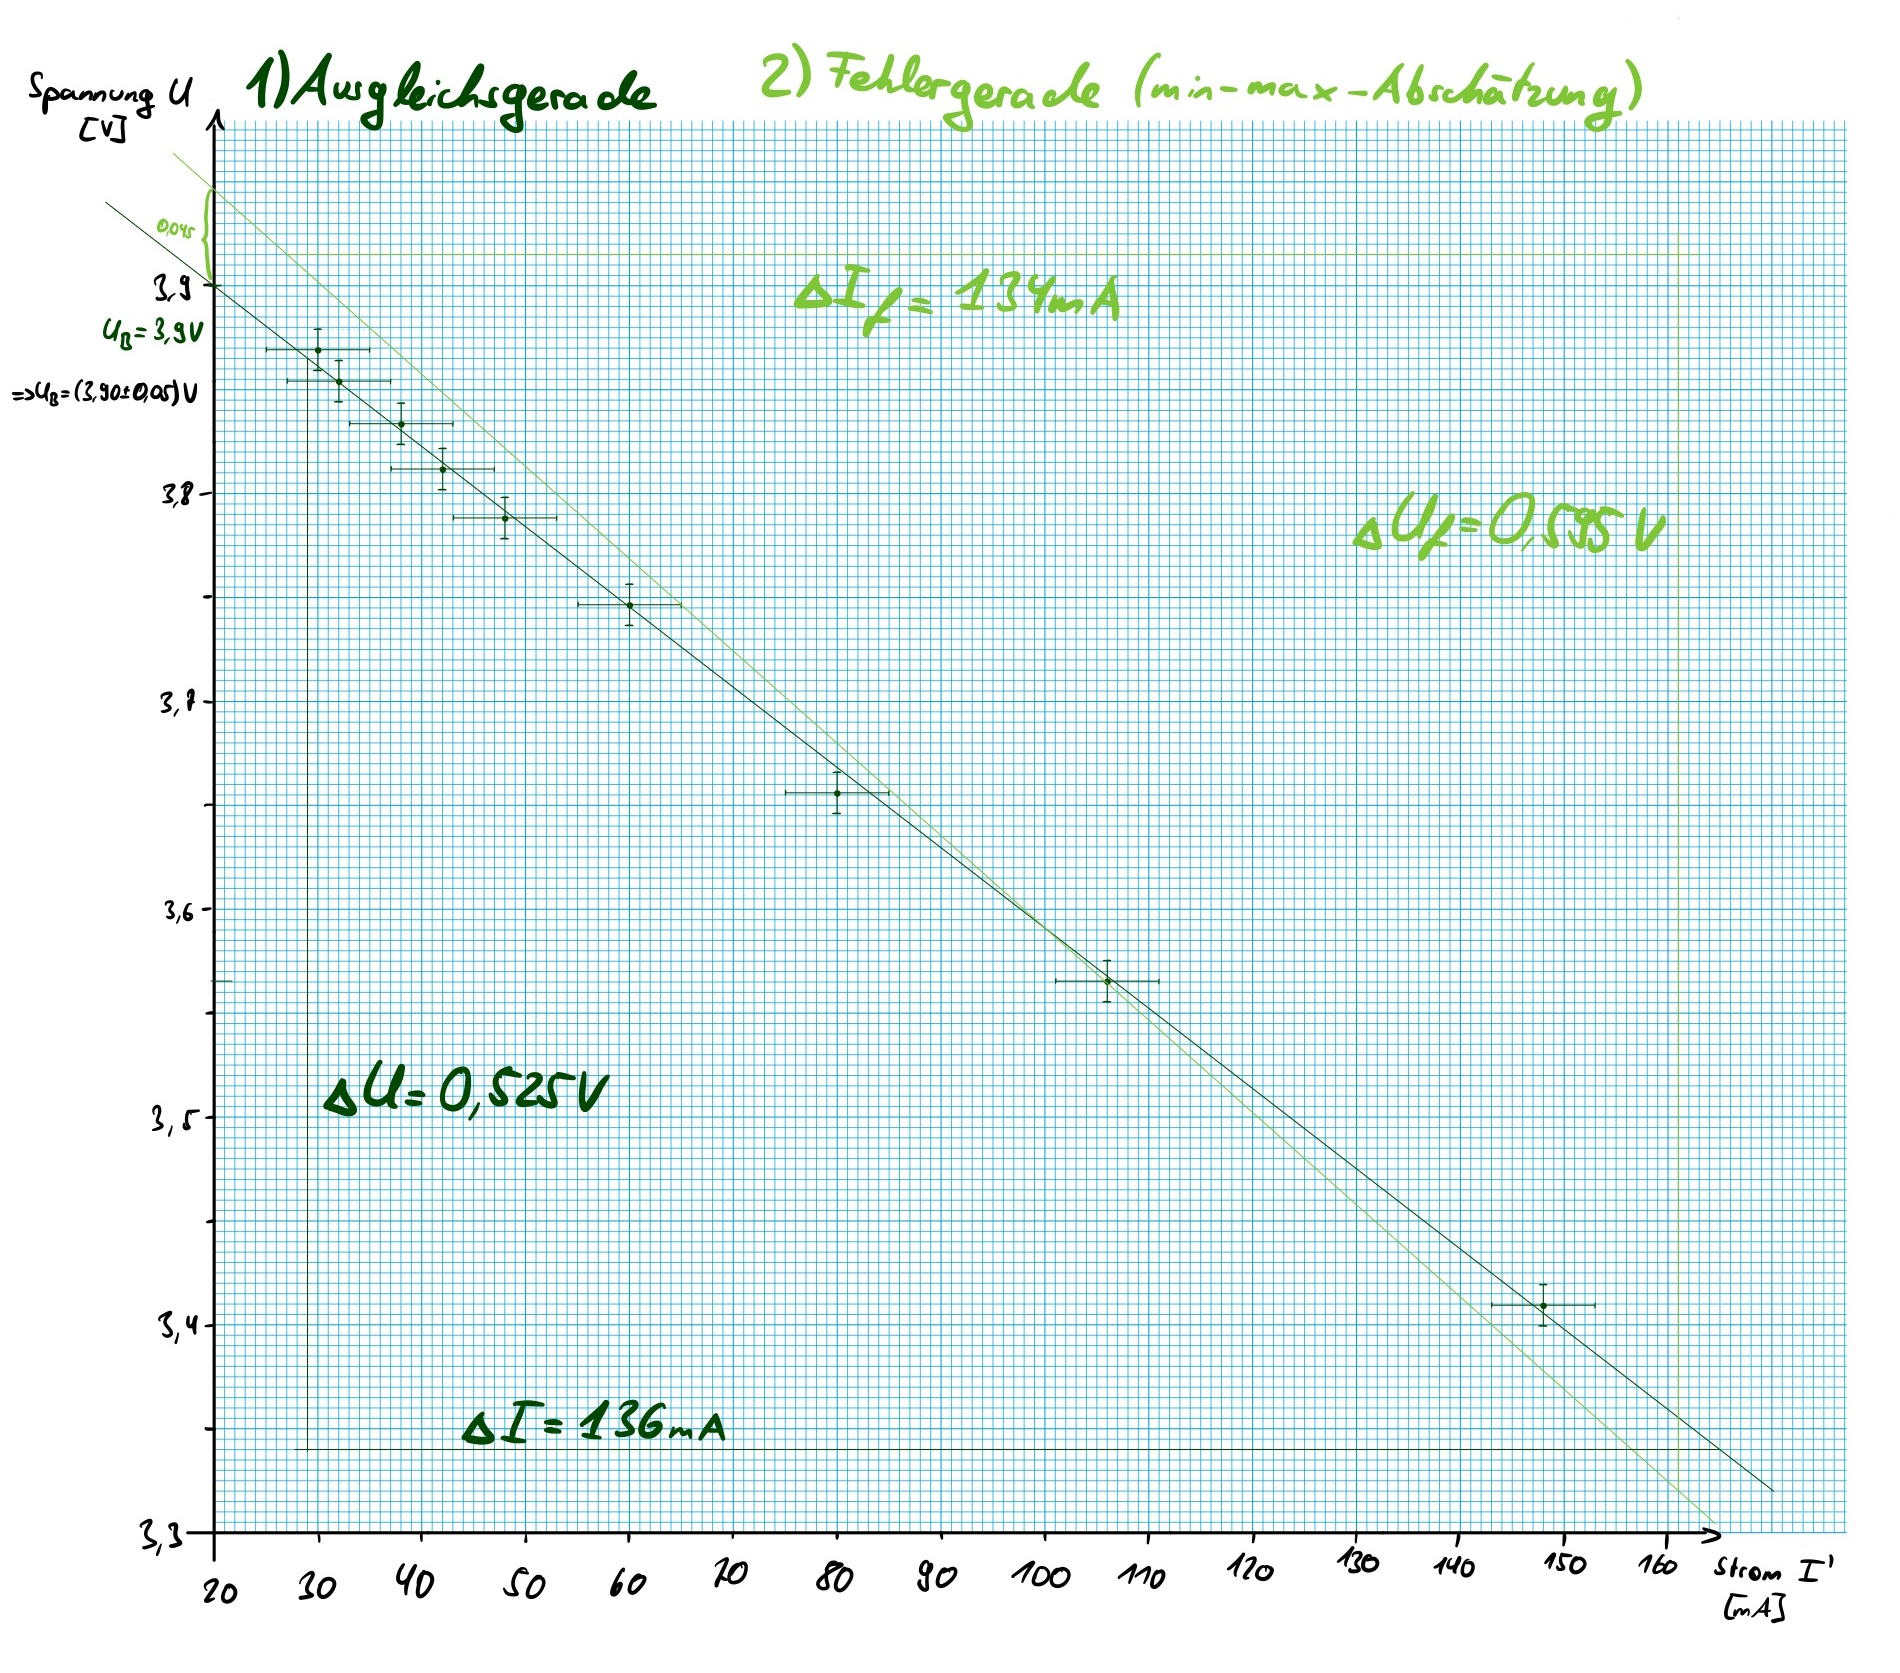
\includegraphics[width=11cm]{graphics/spann.jpg}
    \caption{Spannung als Funktion der Stromstärke}
    \label{fig:spann}
\end{figure}

\newpage

\subsection{Bestimmung des Leistungsmaximums einer Batterie}

Zuletzt möchten wir bestimmen, bei welchem Lastwiderstand die Leistung $P$ einer Batterie am höchsten ist und wie die Spannung dann aussieht. Dazu setzen wir in die Leistungsgleichung $P=UI$ das Ohmsche Gesetz mit dem Lastwiderstand $R_L$ aus Gleichung 3 ein und differenzieren die resultierende Gleichung:

\begin{equation}
    \begin{split}
        P&=UI=R_LI^2 \\
        \implies P(R_L) &= R_L \frac{U_q^2}{(R_I + R_L)^2} \\ 
    \end{split}
\end{equation}

\begin{equation}
    \frac{d}{dR_L} P(R_L) = \Dot{P}(R_L) = \frac{U_q^2}{(R_I + R_L)^2} \left( 1 - \frac{2R_L}{R_I + R_L} \right)
\end{equation}

\bigskip
Um den Wert für $R_L$ zu bestimmen, bei dem $P$ maximal ist, setzten wir die Ableitung gleich 0:

\begin{equation}
    \begin{split}
        0 &= \frac{U_q^2}{(R_I + R_L)^2} \left( 1 - \frac{2R_L}{R_I + R_L} \right) \\
        \iff 0 &= 1 - \frac{2R_L}{R_I + R_L} \\
        \iff R_I &= R_L \\
    \end{split}
\end{equation}

Wir sehen also, dass die Leistung maximal ist, wenn der angeschlossene Lastwiderstand gleich dem Innenwiderstand der Batterie ist. Mit Gleichung 3 für $U$ von oben ergibt sich dann für die Spannung:

\begin{equation}
    U = R_I \frac{U_q}{R_I+R_I} = \frac{U_q}{2}
\end{equation}

\newpage
%---------------PRÄSENTATION DER ENDERGEBNISSE---------------
\section{Präsentation der Endergebnisse}

In diesem Versuch haben wir einen der Steckwiderstände bestimmt als

\begin{equation}
    \bm{R} = \bm{818,18 \Omega}
\end{equation}

und bei Überprüfung der Messungen der beiden Messgeräte auf die Maschenregel festgestellt, dass die des Kompensators die Regel besser erfüllt hat.

Anschließend haben wir die Quellspannung 

\begin{equation}
    \bm{U_B} = \bm{(3,90 \pm 0,05)\textbf{V}}
\end{equation}

sowie den Innenwiderstand der Batterie

\begin{equation}
    \bm{R_i} = \bm{(3,9 \pm 0,6) \Omega}
\end{equation}

bestimmt.

Zuletzt haben wir hergeleitet, dass die Leistung der Batterie am größten wird wenn der angeschlossene Lastwiderstand dem Innenwiderstand entspricht und wie groß die Spannung dann ist:


\begin{equation}
    \bm{U} = \bm{\frac{U_q}{2}}
\end{equation}

\newpage
%---------------ZUSAMMENFASSUNG UND DISKUSSION---------------
\section{Zusammenfassung und Diskussion}

Für ein erstes Kennenlernen der Grundlagen der Elektrotechnik haben wir in diesem Versuch mit verschiedenen Setups Spannungen und Stromstärken gemessen, Messbereicherweiterungen durchgeführt und verschiedene Messgeräte miteinander verglichen. Wir stellten Untersuchungen in den Bereichen Innenwiderstand und Lastwiderstand sowie Quellspannung und Klemmspannung an.

Da in diesem Versuch praktisch keine Literaturwerte oder sonstige ideale Angaben zur Verfügung standen, lässt sich zu den finalen Ergebnissen nur sagen, dass diese im Kontext des Versuchs und den verwendeten Materialien Sinn ergeben. Die bestimmten Spannungen in Teil 2 erzielten überall erwartete Ergebnisse: Die gemessene Spannung von etwa 4V bei beiden Messgeräten aus der Batterie ohne Steckwiderstände lag etwas unter der Angabe von 4,5V, was darauf schließen lässt, dass die Batterie schon etwas leer ist. Genauso ergaben die Spannungsmessungen über die Steckwiderstände sowie die Resultate beim Überprüfen der Maschenregel Sinn: Beim Drehspulinstrument fällt aufgrund des vergleichsweise kleinen Innenwiderstands eine signifikante Spannung über diesem ab, wodurch die gemessenen Spannungen addiert nicht die Maschenregel zu erfüllen schien. Im Gegenzug fällt beim Kompensator aufgrund des sehr hohen Innenwiderstands keine Spannung ab. Beim letzten Teil scheinen die Endergebnisse für die Quellspannung und den Innenwiderstand auch sinnvoll.

Es lassen sich dennoch ein paar Verbesserungsmöglichkeiten und potenzielle Fehlerquellen anmerken.

Zunächst lässt sich die generelle Voraussetzung von Feingefühl beim Bedienen des Kondensators und beim Ablesen der Messwerte nennen. Insbesondere die Skala des Drehspulinstrumeters war teils etwas grob und die Nullstellung des Kompensators etwas knifflig. Beides scheint in Anbetracht der Endergebnisse aber gut von unseren Fehlern aufgefangen zu sein.

Auch lässt sich noch kurz die Ungenauigkeit des grafischen Verfahrens beim Zeichnen des Diagramms $U(I)$ nennen. Manuell per Hand Punkte einzeichnen, Ausgleichsgeraden finden und Fehlergeraden abschätzen ist immer etwas ungenau. Computerbasierte Visualisierungen hätten hier ein genaueres Ergebnis liefern können.

Jedoch kann man allgemein sagen, dass dieser Versuch bis auf Ablesefehler recht fehlersicher ist. Da keine übermäßig großen manuellen Einstellungen von unserer Seite durchgeführt werden mussten, bis auf die Kalibrierung des Kompensators, welche aber genau der Verwendungsweise entspricht und somit nicht wirklich viel komplexer als die spätere Nutzung war, sind hier eigenltlich keine direkten Fehlerquellen vorzufinden. Während des Versuchs beschränkte sich unsere Interaktion auf das Ablesen der Skalen, die Nullstellung des Kompensators und den richtigen Aufbau des Schaltkreises, was alles mit den gegebenen Hilfen immer recht gut funktioniert hat. 

Zusammenfassen lässt sich sagen, dass alle Ergbnisse sinnvoll erscheinen und im Kontext des Versuchs ein zufriedenstellendes Endresultat erzielt werden konnte. Im Endeffekt diente dieser Versuch aber auch mehr dem Kennenlernen und einer ersten Einführung in den Bereich der Stom- und Spannungsmessungen. Auch dieses Ziel konnte unserer Ansicht nach gut erfüllt werden. 

\end{document}

